\counterwithout{figure}{section}

\anonsection{Введение}

IBM Spectrum LSF --- это система очередей задач, позволяющая пользователям запускать задачи на кластере. Кластер состоит из множества вычислительных узлов, каждый из которых имеет набор процессоров ипамять. Пользователь отправляет задачу, в которой указана последовательность команд, которую он хочет запустить, вместе с описанием вычислительных ресурсов, необходимых для исполнения задачи: время, процессор, ядра, узлы \cite{hpc-llnl}.

\begin{figure}[h]
    \centering
    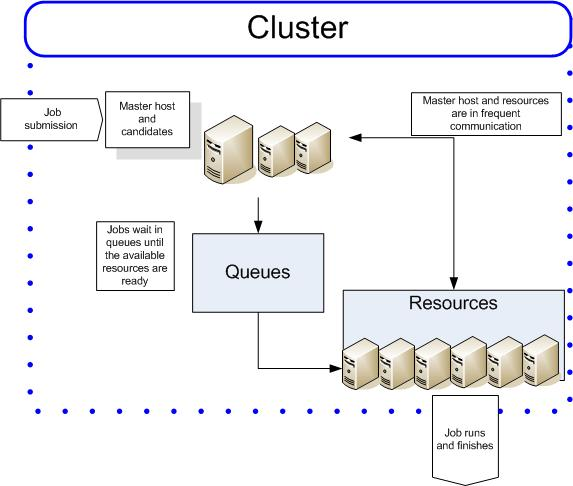
\includegraphics{lsf_cluster_overview.jpg}
    \caption{Кластер LSF}
    \label{fig:LSF_cluster}
\end{figure}

Система очередей задач позволяет распределить пользовательские задачи сети для расчетов гидродинамических моделей с различными запрашиваемыми ресурсами: кол-во ядер, кол-во и тип узлов.

Приложение клиент Scheduler позволяет пользователям рассчитывать на сервере кластере гидродинамические модели. В нем поддерживаются системы очередей: Torque, PBS Pro, Slurm. В рамках курсовой работы была поставлена задача поддержки системы очередей IBM Spectrum LSF, поскольку кластеры различаются и у них могут быть установлены различные системы очередей.

\clearpage

\counterwithin{figure}{section}